\documentclass[letterpaper]{article} % DO NOT CHANGE THIS
\usepackage{aaai24}  % DO NOT CHANGE THIS
\usepackage{times}  % DO NOT CHANGE THIS
\usepackage{helvet}  % DO NOT CHANGE THIS
\usepackage{courier}  % DO NOT CHANGE THIS
\usepackage[hyphens]{url}  % DO NOT CHANGE THIS
\usepackage{graphicx} % DO NOT CHANGE THIS
\urlstyle{rm} % DO NOT CHANGE THIS
\def\UrlFont{\rm}  % DO NOT CHANGE THIS
\usepackage{natbib}  % DO NOT CHANGE THIS AND DO NOT ADD ANY OPTIONS TO IT
\usepackage{caption} % DO NOT CHANGE THIS AND DO NOT ADD ANY OPTIONS TO IT
\frenchspacing  % DO NOT CHANGE THIS
\setlength{\pdfpagewidth}{8.5in} % DO NOT CHANGE THIS
\setlength{\pdfpageheight}{11in} % DO NOT CHANGE THIS

\usepackage[dvipsnames]{xcolor}
\usepackage{paralist}
\usepackage{enumitem}
\usepackage{multirow}
\usepackage{amsmath}
\usepackage{amsthm}
\usepackage{amssymb}
\usepackage{graphicx}
\usepackage{subcaption}
\usepackage{comment}
\usepackage{nicefrac}
\usepackage{booktabs}
\newtheorem{prop}{Proposition}
\newtheorem{thm}{Theorem}
\allowdisplaybreaks

\input{math_commands.tex}
\def\R{\mathbb{R}}
\def\ba{\mathbf{a}}
\newcommand{\abs}[1]{\left|#1\right|}
\newcommand{\norm}[1]{\left\|#1\right\|}
\newcommand{\prob}[1]{\operatorname{Pr}\left(#1\right)}
\newcommand{\expec}[1]{\operatorname{E}\left[#1\right]}
\newcommand{\size}[1]{\left|#1\right|}
\newcommand{\inner}[2]{\left\langle #1, #2\right\rangle}


\begin{comment}
\usepackage{newfloat}
\usepackage{listings}
\DeclareCaptionStyle{ruled}{labelfont=normalfont,labelsep=colon,strut=off} % DO NOT CHANGE THIS
\lstset{%
	basicstyle={\footnotesize\ttfamily},% footnotesize acceptable for monospace
	numbers=left,numberstyle=\footnotesize,xleftmargin=2em,% show line numbers, remove this entire line if you don't want the numbers.
	aboveskip=0pt,belowskip=0pt,%
	showstringspaces=false,tabsize=2,breaklines=true}
\floatstyle{ruled}
\newfloat{listing}{tb}{lst}{}
\floatname{listing}{Listing}
\end{comment}



\setcounter{secnumdepth}{2} %May be changed to 1 or 2 if section numbers are desired.



\iffalse
\title{Rethinking Robustness of Model Attributions}
\author{
    Sandesh Kamath,
    Sankalp Mittal,\\
    Amit Deshpande,
    Vineeth Balasubramanian
}
\affiliations{
    \textsuperscript{\rm 1}Indian Institute of Technology, Hyderabad\\
    \textsuperscript{\rm 2}Microsoft Research, Bengaluru\\

    Sandesh Kamath\textsuperscript{\rm 1},
    Sankalp Mittal\textsuperscript{\rm 1},
    Amit Deshpande\textsuperscript{\rm 2},
    Vineeth N Balasubramanian\textsuperscript{\rm 1}
    sandesh.kamath@gmail.com
}
\fi

\iffalse
\title{My Publication Title --- Single Author}
\author {
    Author Name
}
\affiliations{
    Affiliation\\
    Affiliation Line 2\\
    name@example.com
}
\fi

\title{Rethinking Robustness of Model Attributions}
\author {
    Sandesh Kamath\textsuperscript{\rm 1},
    Sankalp Mittal\textsuperscript{\rm 1},
    Amit Deshpande\textsuperscript{\rm 2},
    Vineeth N Balasubramanian\textsuperscript{\rm 1}
}
\affiliations {
    \textsuperscript{\rm 1}Indian Institute of Technology, Hyderabad\\
    \textsuperscript{\rm 2}Microsoft Research, Bengaluru\\
    sandesh.kamath@gmail.com,
}



\begin{document}

\maketitle

\begin{abstract}
For machine learning models to be reliable and trustworthy, their decisions must be interpretable. As these models find increasing use in safety-critical applications, it is important that not just the model predictions but also their explanations (as feature attributions) be robust to small human-imperceptible input perturbations. Recent works have shown that many attribution methods are fragile and have proposed improvements in either these methods or the model training. We observe two main causes for fragile attributions: first, the existing metrics of robustness (e.g., top-$k$ intersection) overpenalize even reasonable local shifts in attribution, thereby making random perturbations to appear as a strong attack, and second, the attribution can be concentrated in a small region even when there are multiple important parts in an image. To rectify this, we propose simple ways to strengthen existing metrics and attribution methods that incorporate locality of pixels in robustness metrics and diversity of pixel locations in attributions. Towards the role of model training in attributional robustness, we empirically observe that adversarially trained models have more robust attributions on smaller datasets, however, this advantage disappears in larger datasets. Code is made available\footnote{https://github.com/ksandeshk/LENS}.

\end{abstract}

\section{Introduction}
\label{sec_intro}
The explosive increase in the use of deep neural network (DNN)-based models for applications across domains has resulted in a very strong need to find ways to interpret the decisions made by these models \citep{GadeGKMT20,Tang2021shap,Yap2021rna,Oviedo2022,OhJ20a}. Interpretability is an important aspect of responsible and trustworthy AI, and model explanation methods (also known as attribution methods) are an important aspect of the community's efforts towards explaining and debugging real-world AI/ML systems. %Attribution methods are used across application domains today \citep{GadeGKMT20,Tang2021shap,Yap2021rna,Oviedo2022,OhJ20a}, despite their limitations. %Instead of using the model as a black box, efforts have been made to find approaches to explain the decisions made by these models
Attribution methods \citep{zeiler2015deconv,simonyan2014deep,bach2015lrp,Selvaraju_2019,Chattopadhay_2018,SundararajanTY17,shrikumar2017just,smilkov2017smoothgrad,lundberg2017unified} attempt to explain the decisions made by DNN models through input-output attributions or saliency maps. \citep{lipton2018mythos,samek_explainable_2019,fan_interpretability_2021,zhang_survey_2020} present detailed surveys on these methods. %, instead of using them as a black box.
Recently, the growing numbers of attribution methods has led to a concerted focus on studying the robustness of attributions to input perturbations to handle potential security hazards \citep{chen2019robust,sarkar2020enhanced, Wang22Kendall, agarwal2022rethinking}. One could view these efforts as akin to adversarial robustness that focuses on defending against attacks on model predictions, whereas \textit{attributional robustness} focuses on defending against attacks on model explanations.
For example, an explanation for a predicted credit card failure cannot change significantly for a small human-imperceptible change in input features, or the saliency maps explaining the COVID risk prediction from a chest X-ray should not change significantly with a minor human-imperceptible change in the image. %This is referred to as attributional robustness.

DNN-based models are known to have a vulnerability to imperceptible adversarial perturbations \citep{Biggio_2013,szegedy2014intriguing,goodfellow15fgsm}, which make them misclassify input images. %These small imperceptible perturbations are constructed using techniques like Fast Gradient Signed Method (FGSM) \citep{goodfellow15fgsm} and Projected Gradient Descent (PGD) \citep{madry2019deep}. %PGD \citep{madry2019deep} is currently the strongest adversarial attack.
Adversarial training \citep{madry2019deep} is widely understood to provide a reasonable degree of robustness to such perturbation attacks.
While adversarial robustness has received significant attention over the last few years \citep{ozdag2018advsurvey,silva2020advrobustsurvey}, the need for stable and robust attributions, corresponding explanation methods and their awareness are still in their early stages at this time \citep{ghorbani2018interpretation,chen2019robust,slack2020fooling,sarkar2020enhanced,lakkaraju2020icml,slack2021neurips-a,slack2021neurips-b}. In an early effort, \citep{ghorbani2018interpretation} provided a method to construct a small imperceptible perturbation which when added to an input $x$ results in a change in attribution map of the original map to that of the perturbed image. This is measured through top-$k$ intersection, Spearman's rank-order correlation or Kendall's rank-order correlation between the two attribution maps (of original and perturbed images). See Figure \ref{fig_intro} for an example. Defenses proposed against such attributional attacks %have also been proposed by regularizing the loss function or by using smoothing techniques on gradients
\citep{chen2019robust,singh2020attributional,wang2020smoothed,sarkar2020enhanced}
also leverage the same metrics to evaluate the robustness of attribution methods.
\begin{figure}[!ht]
  \begin{center}
    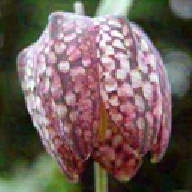
\includegraphics[width=0.15\textwidth]{./images/flower_10_image_pert.pdf}
    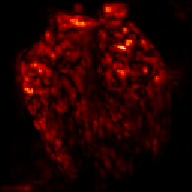
\includegraphics[width=0.15\textwidth]{./images/flower_10_topk_nat_orig.pdf}
    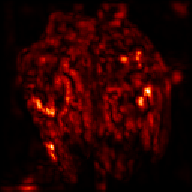
\includegraphics[width=0.15\textwidth]{./images/flower_10_topk_nat_pert.pdf}\\
    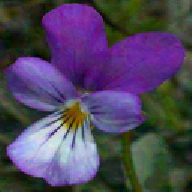
\includegraphics[width=0.15\textwidth]{./images/flower_4_image_pert.pdf}
    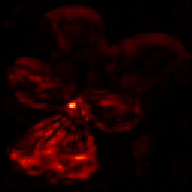
\includegraphics[width=0.15\textwidth]{./images/flower_4_topk_nat_orig.pdf}
    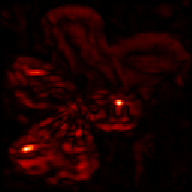
\includegraphics[width=0.15\textwidth]{./images/flower_4_topk_nat_pert.pdf}\\
    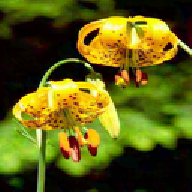
\includegraphics[width=0.15\textwidth]{./images/flower_18_image_pert.pdf}
    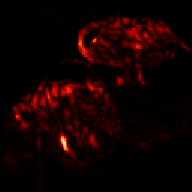
\includegraphics[width=0.15\textwidth]{./images/flower_18_topk_nat_orig.pdf}
    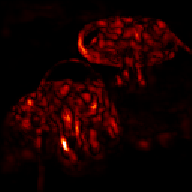
\includegraphics[width=0.15\textwidth]{./images/flower_18_topk_nat_pert.pdf}
  \end{center}
  \caption{Sample images from Flower dataset with Integrated Gradients (IG) before and after attributional attack. The attack used here is the top-$k$ attributional attack of \citet{ghorbani2018interpretation} on a ResNet model. Robustness of attribution measured by top-$k$ intersection is small, and ranges from 0.04 (first image) to 0.45 (third image) as it penalizes for both local changes in attribution and concentration of top pixels in a small region. Visually, we can observe that such overpenalization leads to a wrong sense of robustness as the changes are within the object of importance.}
  \label{fig_intro}
\end{figure}

While these efforts have showcased the need and importance of studying the robustness of attribution methods, we note in this work that the metrics used, and hence the methods, can be highly sensitive to minor local changes in attributions (see Fig \ref{fig_intro} \textit{row 2}).
We, in fact, show (in Appendix \ref{app:subsec:rand-vec}) that under existing metrics to evaluate robustness of attributions, a random perturbation can be as strong an attributional attack as existing benchmark methods. This may not be a true indicator of the robustness of a model's attributions, and can mislead further research efforts in the community. We hence focus our efforts in this work on rethinking metrics and methods to study the robustness of model attributions (in particular, we study image-based attribution methods to have a focused discussion and analysis). Beyond highlighting this important issue, we propose locality-sensitive improvements of the above metrics that incorporate the locality of attributions along with their rank order. We show that such a locality-sensitive distance is upper-bounded by a metric based on symmetric set difference. We also introduce a new measure {\bf top-$k$-div} that incorporates diversity of a model's attributions. % in the top-$k$ pixels picked. And show that infusing diversity and locality to observe the change between the explanation maps could be a better approach, thus providing an improved sense of attribution robustness. %One could also view existing methods that attempt to achieve attributional robusthe robust attribution methods proposed in recent works also reflect this premise of locality, thus highlighting the need for a locality-sensitive metric for progress in the field. %Our empirical results on well-known benchmark datasets using well-known models and attribution methods support our observations and conclusions in this work.
Our key contributions are summarized below:
\begin{itemize}[leftmargin=*]
\setlength\itemsep{-0.06em}
\item Firstly, we observe that existing robustness metrics for model attributions overpenalize minor drifts in attribution, leading to a false sense of fragility. %We go on to show that under existing such metrics, a random perturbation is as good an attack as principled methods like \citet{ghorbani2018interpretation}.
\item In order to address this issue, we propose Locality-sENSitive (LENS) improvements of existing metrics, namely, LENS-top-$k$, LENS-Spearman and LENS-Kendall, that incorporate the locality of attributions along with their rank order. Besides avoiding overpenalizing attribution methods for minor local drifts, we show that our proposed LENS variants are well-motivated by metrics defined on the space of attributions. %, and provide tighter bounds on the attributional robustness of already known improvements in attribution methods and model training designed for better attributions.
\item We subsequently introduce a second measure based on diversity that enriches model attributions by preventing the localized grouping of top model attributions. LENS can be naturally applied to this measure, thereby giving a method to incorporate both diversity and locality in measuring attributional robustness.
\item Our comprehensive empirical results on benchmark datasets and models used in existing work clearly support our aforementioned observations, as well as the need to rethink the evaluation of the robustness of model attributions using locality and diversity.
\item Finally, we also show that existing methods for robust attributions implicitly support such a locality-sensitive metric for evaluating progress in the field.
\end{itemize}
\section{Background and Related Work}
\label{sec_related_work}
We herein discuss background literature from three different perspectives that may be related to our work: model explanation/attribution methods, efforts on attributional robustness (both attacks and defenses), and other recent related work.
\noindent \textbf{Attribution Methods.} Existing efforts on explainability in DNN models can be broadly categorized as: local and global methods, model-agnostic and model-specific methods, or as post-hoc and ante-hoc (intrinsically interpretable) methods \citep{molnar2019,xaitutorial}. Most existing methods in use today -- including methods to visualize weights and neurons \citep{simonyan2014deep,ZeilerF14}, guided backpropagation \citep{springenberg2015striving}, CAM \citep{ZhouKLOT16}, GradCAM \citep{Selvaraju_2019}, Grad-CAM++ \citep{Chattopadhay_2018}, LIME \citep{ribeiro2016why}, DeepLIFT \citep{shrikumar2017just,shrikumar2019learning}, LRP \citep{bach2015lrp}, Integrated Gradients \citep{SundararajanTY17}, SmoothGrad \citep{smilkov2017smoothgrad}), DeepSHAP \citep{lundberg2017unified} and TCAV \citep{kim2018interpretability} -- are post-hoc methods, which are used on top of a pre-trained DNN model to explain its predictions. We focus on such post-hoc attribution methods in this work. For a more detailed survey of explainability methods for DNN models, please see \citep{xaitutorial,molnar2019,samek_explainable_2019}.

\noindent \textbf{Robustness of Attributions.} The growing numbers of attribution methods proposed has also led to efforts on identifying the desirable characteristics of such methods \citep{alvarez2018robustness,AdebayoGMGHK18,yeh2019fidelity,ChalasaniC00J20,TomsettHCGP20,Boggust22Faithful,agarwal2022rethinking}. A key desired trait that has been highlighted by many of these efforts is robustness or stability of attributions, i.e., the explanation should not vary significantly within a small local neighborhood of the input \citep{alvarez2018robustness,ChalasaniC00J20}. \citet{ghorbani2018interpretation} showed that well-known methods such as gradient-based attributions, DeepLIFT \citep{shrikumar2019learning} and Integrated Gradients (IG) \citep{SundararajanTY17} are vulnerable to such input perturbations, and also provided an algorithm to construct a small imperceptible perturbation which when added to the input results in changes in the attribution.  \citet{slack2020fooling} later showed that methods like LIME \citep{ribeiro2016why} and DeepSHAP \citep{lundberg2017unified} are also vulnerable to such manipulations. The identification of such vulnerability and potential for attributional attacks has since led to multiple research efforts to make a model's attributions robust. \citet{chen2019robust} proposed a regularization-based approach, where an explicit regularizer term is added to the loss function to maintain the model gradient across input (IG, in particular) while training the DNN model. This was subsequently extended by \citep{sarkar2020enhanced,singh2020attributional,wang2020smoothed}, all of whom provide different training strategies and regularizers to improve attributional robustness of models. Each of these methods including \citet{ghorbani2018interpretation} measures change in attribution before and after input perturbation using the same metrics: top-$k$ intersection, and/or rank correlations like Spearman's $\rho$ and Kendall' $\tau$. Such metrics have recently, in fact, further been used to understand issues surrounding attributional robustness \citep{Wang22Kendall}. Other efforts that quantify stability of attributions in tabular data also use Euclidean distance (or its variants) between the original and perturbed attribution maps  \citep{alvarez2018robustness,yeh2019fidelity,agarwal2022rethinking}. Each of these metrics look for dimension-wise correlation or pixel-level matching between attribution maps before and after perturbation, and thus penalize even a minor change in attribution (say, even by one pixel coordinate location). This results in a false sense of fragility, and could even be misleading. In this work, we highlight the need to revisit such metrics, and propose variants based on locality and diversity that can be easily integrated into existing metrics.

\noindent \textbf{Other Related Work.} In other related efforts that have studied similar properties of attribution-based explanations, \citep{carvalho2019machine,bhatt2020evaluating} stated that stable explanations should not vary too much between similar input samples, unless the model's prediction changes drastically. The abovementioned attributional attacks and defense methods \citep{ghorbani2018interpretation,sarkar2020enhanced,singh2020attributional,wang2020smoothed} maintain this property, since they focus on input perturbations that change the attribution without changing the model prediction itself. Similarly, \citet{arun2020assessing} and \citet{fel2022good} introduced the notions of repeatability/reproducibility and generalizability respectively, both of which focus on the desired property that a trustworthy explanation must point to similar evidence across similar input images. In this work, we provide a practical metric to study this notion of similarity by considering locality-sensitive metrics.
\section{{\bf L}ocality-s{\bf ENS}itive Metrics (LENS) for Attributional Robustness} \label{sec:lens}
 \begin{figure}[h]
 \centering
     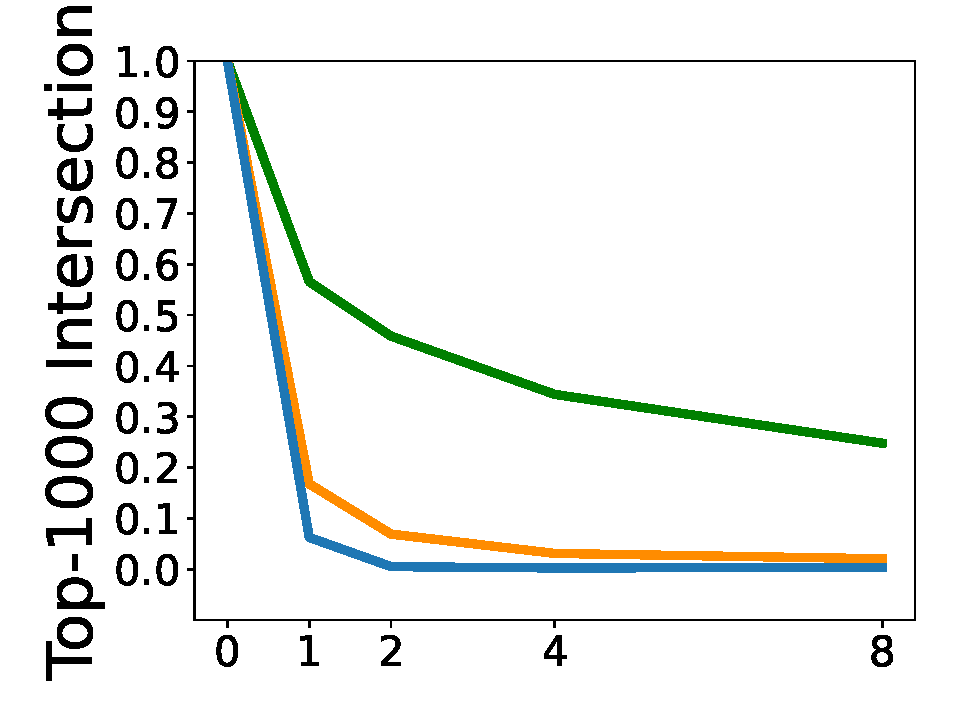
\includegraphics[width=0.22\textwidth]{./plots/imagenet_gh_lens_sg_orig_pert_all.pdf}
     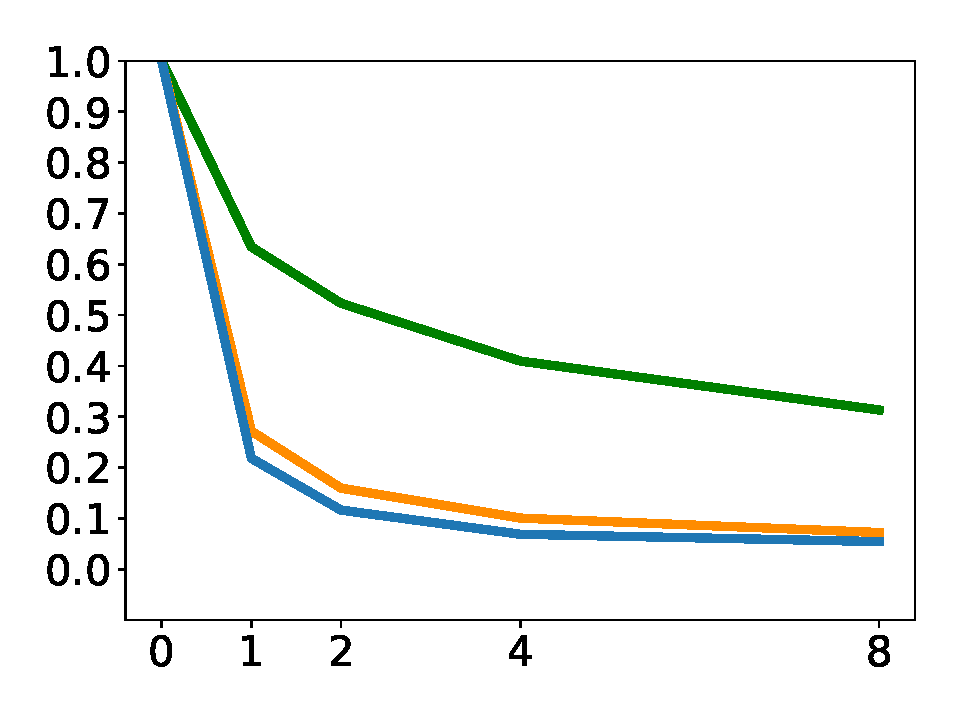
\includegraphics[width=0.22\textwidth]{./plots/imagenet_gh_lens_ig_orig_pert_all.pdf}\\
     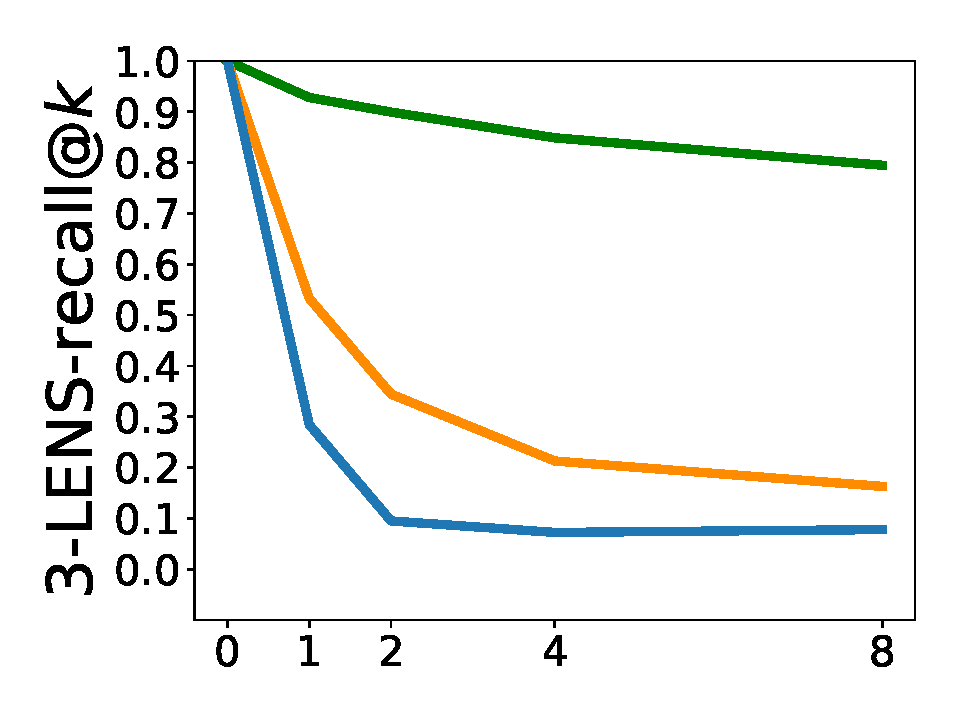
\includegraphics[width=0.22\textwidth]{./plots/imagenet_gh_lens_sg_orig_pert_all_lens.pdf}
     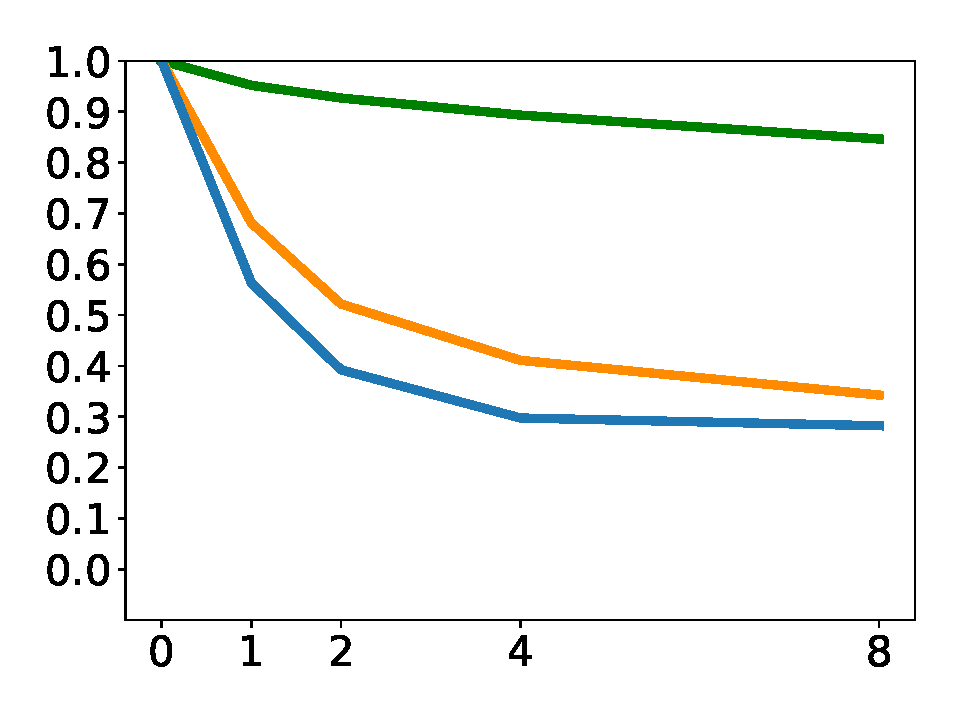
\includegraphics[width=0.22\textwidth]{./plots/imagenet_gh_lens_ig_orig_pert_all_lens.pdf}\\
     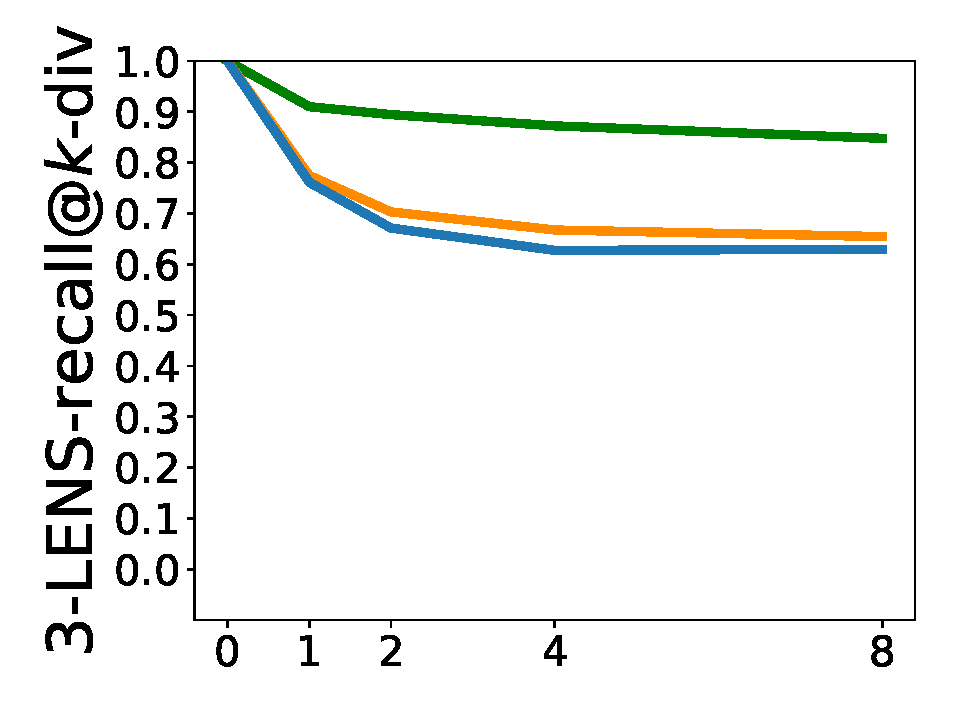
\includegraphics[width=0.22\textwidth]{./plots/imagenet_gh_lens_sg_orig_pert_all_div.pdf}
     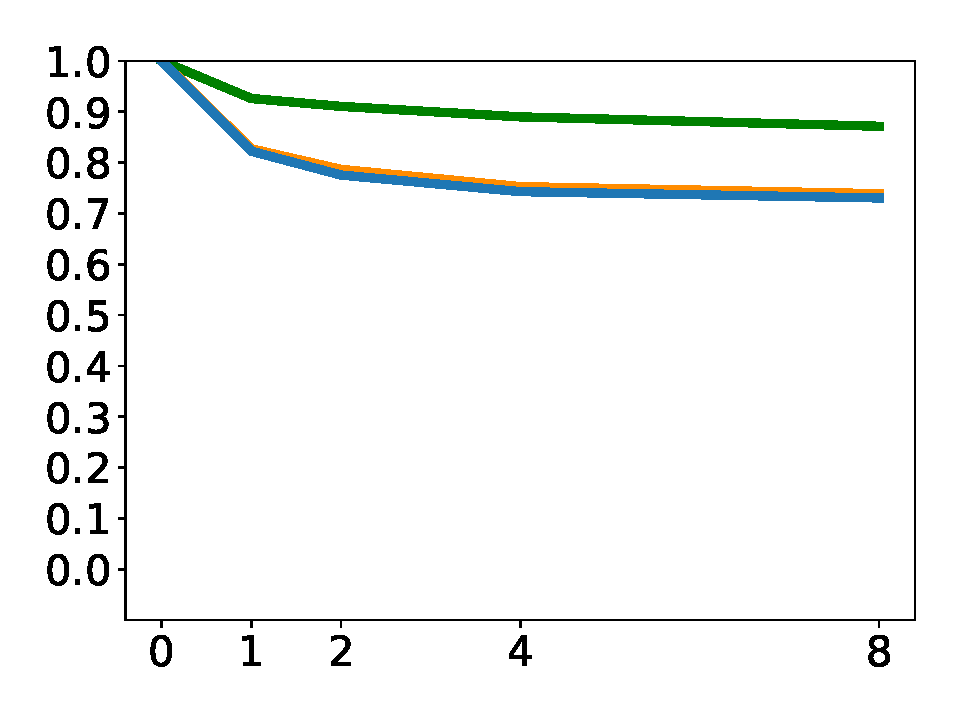
\includegraphics[width=0.22\textwidth]{./plots/imagenet_gh_lens_ig_orig_pert_all_div.pdf}
    \caption{From top to bottom, we plot average top-$k$ intersection (currently used metric), $3$-LENS-recall@$k$ and $3$-LENS-recall@$k$-div (proposed metrics) against the $\ell_{\infty}$-norm of  attributional attack perturbations for Simple Gradients (SG) (left) and Integrated Gradients (IG) (right) of a SqueezeNet model on Imagenet. We use $k=1000$ and three attributional attack variants proposed by \citet{ghorbani2018interpretation}. Evidently, the proposed metrics show more robustness under the same attacks.}
\label{imagenet-ghorbani-with-lens-div}
\end{figure}

As a motivating example, Figure \ref{imagenet-ghorbani-with-lens-div} presents the results obtained using \cite{ghorbani2018interpretation} with Simple Gradients (SG) and Integrated Gradients (IG) of an NN model trained on ImageNet. The top row, which reports the currently followed top-$k$ intersection measure of attribution robustness, shows a significant drop in robustness performance even for the random sign attack (green line). The subsequent rows, which report our metrics for the same experiments, show significant improvements in robustness -- especially when combining the notions of locality and diversity. Observations made on current metrics could lead to a false sense of fragility, which overpenalizes even an attribution shift by 1-2 pixels. A detailed description of our experimental setup for these results is available in Appendix \ref{app:exp-setup}. Motivated by these observations, we explore improved measures for attributional robustness that maintain the overall requirements of robustness, but do not overpenalize minor deviations.
\begin{figure}[!ht]
  \begin{center}
    
\includegraphics[width=0.11\textwidth]{./images/flower_19_image.pdf}
    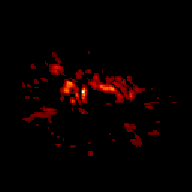
\includegraphics[width=0.11\textwidth]{./images/flower_19_topk_nat_orig_orig.pdf}
    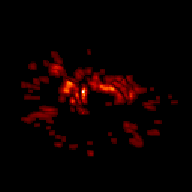
\includegraphics[width=0.11\textwidth]{./images/flower_19_topk_nat_orig_lens_rec.pdf}
    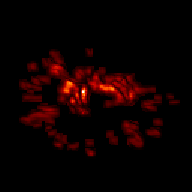
\includegraphics[width=0.11\textwidth]{./images/flower_19_topk_nat_orig_2lens_rec.pdf}\\
    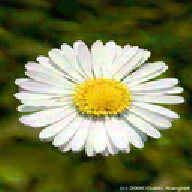
\includegraphics[width=0.11\textwidth]{./images/flower_19_image_pert.pdf}
    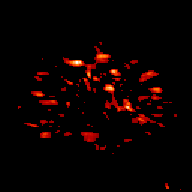
\includegraphics[width=0.11\textwidth]{./images/flower_19_topk_nat_orig_pert.pdf}
    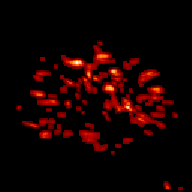
\includegraphics[width=0.11\textwidth]{./images/flower_19_topk_nat_orig_lens_pre.pdf}
    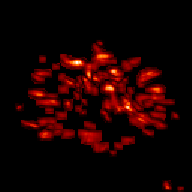
\includegraphics[width=0.11\textwidth]{./images/flower_19_topk_nat_orig_2lens_pre.pdf}\\
  \end{center}
      \caption{A sample image from Flower dataset before (top) and after (bottom) the top-$k$ attributional attack of \cite{ghorbani2018interpretation} on a ResNet model for Integrated Gradients (IG) attribution method. From left to right: the image, its top-$k$ pixels as per IG, the union of the $3 \times 3$-pixel neighborhoods and $5 \times 5$-pixel neighborhoods of the top-$k$ pixels, respectively, for $k=1000$. Quantitatively, top-$k$ intersection: 0.14, 1-LENS-recall@$k$: 0.25, 1-LENS-pre@$k$: 0.37, 2-LENS-recall@$k$: 0.40, 2-LENS-pre@$k$: 0.62.} %\textit{Zoom images for finer details.}}
    \label{fig_intro_lens-19}
\end{figure}
\subsection{Defining LENS Metrics for Attributions} \label{subsec:define-lens}
To begin with, we propose an extension of existing similarity measures to incorporate the locality of pixel attributions in images to derive more practical and useful measures of attributional robustness. Let $a_{ij}(x)$ denote the attribution value or importance assigned to the $(i, j)$-th pixel in an input image $x$, and let $S_{k}(x)$ denote the set of $k$ pixel positions with the largest attribution values. Let $N_{w}(i, j) = \{(p, q) \;:\; i-w \leq p \leq i+w,~ j-w \leq q \leq j+w\}$ be the neighboring pixel positions within a $(2w+1) \times (2w+1)$ window around the $(i, j)$-th pixel. By a slight abuse of notation, we use $N_{w}(S_{k}(x))$ to denote $\bigcup_{(i, j) \in S_{k}(x)} N_{w}(i, j)$, that is, the set of all pixel positions that lie in the union of $(2w+1) \times (2w+1)$ windows around the top-$k$ pixels.

For a given attributional perturbation $\mathrm{Att}(\cdot)$, let $T_{k} = S_{k}(x + \mathrm{Att}(x))$ denote the top-$k$ pixels in attribution values after applying the attributional perturbation $\mathrm{Att}(x)$. The currently used top-$k$ intersection metric is then computed as: $\size{S_{k}(x) \cap T_{k}(x)}/k$. To address the abovementioned issues, we instead propose \emph{Locality-sENSitive top-$k$} metrics (LENS-top-$k$) as $\size{N_{w}(S_{k}(x)) \cap T_{k}(x)}/k$ and $\size{S_{k}(x) \cap N_{w}(T_{k}(x))}/k$, which are also closer to more widely used metrics such as precision and recall in ranking methods. We simiarly define Locality-sENSitive Spearman's $\rho$ (LENS-Spearman) and Locality-sENSitive Kendall's $\tau$ (LENS-Kendall) metrics as rank correlation coefficients for the smoothed ranking orders according to $\tilde{a}_{ij}(x)$'s and $\tilde{a}_{ij}(x + \mathrm{Att}(x))$'s, respectively. These can be used to compare two different attributions for the same image, the same attribution method on two different images, or even two different attributions on two different images, as long as the attribution vectors lie in the same space, e.g., images of the same dimensions where attributions assign importance values to pixels. Figure \ref{fig_intro_lens-19} provides the visualization of the explanation map of a sample from the Flower dataset with the top-1000 pixels followed by the corresponding maps with 1-LENS@$k$ and 2-LENS@$k$.

We show that the proposed locality-sensitive variants of the robustness metrics also possess some theoretically interesting properties. Let $\ba_{1}$ and $\ba_{2}$ be two attribution vectors for two images, and let $S_{k}$ and $T_{k}$ be the set of top $k$ pixels in these images according to $\ba_{1}$ and $\ba_{2}$, respectively. We define a locality-sensitive top-$k$ distance between two attribution vectors $\ba_{1}$ and $\ba_{2}$ as $d_{k}^{(w)}(\ba_{1}, \ba_{2})\overset{\text{def}}{=} \text{prec}_{k}^{(w)}(\ba_{1}, \ba_{2}) + \text{recall}_{k}^{(w)}(\ba_{1}, \ba_{2})$, where
$
\text{prec}_{k}^{(w)}(\ba_{1}, \ba_{2}) \overset{\text{def}}{=} \frac{\size{S_{k} \setminus N_{w}(T_{k})}}{k} \quad \text{and}
$
$
\quad \text{recall}_{k}^{(w)}(\ba_{1}, \ba_{2}) \overset{\text{def}}{=} \frac{\size{T_{k} \setminus N_{w}(S_{k})}}{k},
$
similar to precision and recall used in ranking literature, with the key difference being the inclusion of neighborhood items based on locality. Below we state a monotonicity property of $d_{k}^{(w)}(\ba_{1}, \ba_{2})$ and upper bound it in terms of the symmetric set difference of top-$k$ attributions.
\begin{prop} \label{prop:monotone}
For any $w_{1} \leq w_{2}$, we have $d_{k}^{(w_{2})}(\ba_{1}, \ba_{2}) \leq d_{k}^{(w_{1})}(\ba_{1}, \ba_{2}) \leq \size{S_{k} \triangle T_{k}}/k$, where $\triangle$ denotes the symmetric set difference, i.e., $A \triangle B = (A \setminus B) \cup (B \setminus A)$.
\end{prop}
Combining $d_{k}^{(w)}(\ba_{1}, \ba_{2})$ across different values of $k$ and $w$, we can define a distance
\[
d(\ba_{1}, \ba_{2}) = \sum_{k=1}^{\infty} \alpha_{k} \sum_{w=0}^{\infty} \beta_{w}~ d_{k}^{(w)}(\ba_{1}, \ba_{2}),
\]
where $\alpha_{k}$ and $\beta_{w}$ be non-negative weights, monotonically decreasing in $k$ and $w$, respectively, such that $\sum_{k} \alpha_{k} < \infty$ and $\sum_{w} \beta_{w} < \infty$. We show that the distance defined above is upper-bounded by a metric similar to those proposed in \cite{fagin2003comparing} based on symmetric set difference of top-$k$ ranks to compare two rankings.
\begin{prop} \label{prop:metric}
$d(\ba_{1}, \ba_{2})$ defined above is upper-bounded by $u(\ba_{1}, \ba_{2})$ given by
\[
u(\ba_{1}, \ba_{2}) = \sum_{k=1}^{\infty} \alpha_{k} \sum_{w=0}^{\infty} \beta_{w}~ \frac{\size{S_{k} \triangle T_{k}}}{k},
\]
and $u(\ba_{1}, \ba_{2})$ defines a bounded metric on the space of attribution vectors.
\end{prop}
Note that top-$k$ intersection, Spearman's $\rho$ and Kendall's $\tau$ do not take the attribution values $a_{ij}(x)$'s into account but only the rank order of pixels according to these values. We also define a locality-sensitive $w$-smoothed attribution as follows.
\[
\tilde{a}_{ij}^{(w)}(x) = \frac{1}{(2w+1)^{2}} \sum_{\substack{(p, q) \in N_{w}(i, j), \\ 1 \leq p, q \leq n}} a_{pq}(x)
\]
We show that the $w$-smoothed attribution leads to a contraction in the $\ell_{2}$ norm commonly used in theoretical analysis of simple gradients as attributions.
\begin{prop} \label{prop:w-smoothed}
For any inputs $x, y$ and any $w \geq 0$, $\norm{\tilde{\ba}^{(w)}(x) - \tilde{\ba}^{(w)}(y)}_{2} \leq \norm{\ba(x) - \ba(y)}_{2}$.
\end{prop}
Thus, any theoretical bounds on the attributional robustness of simple gradients in $\ell_{2}$ norm proved in previous works continue to hold for locality-sensitive $w$-smoothed gradients. For example, \cite{wang2020smoothed} show the following Hessian-based bound on simple gradients. For an input $x$ and a classifier or model defined by $f$, let $\nabla_{x}(f)$ and $\nabla_{y}(f)$ be the simple gradients w.r.t. the inputs at $x$ and $y$. Theorem 3 in \cite{wang2020smoothed} upper bounds the $\ell_{2}$ distance between the simple gradients of nearby points $\norm{x - y}_{2} \leq \delta$ as  $\norm{\nabla_{x}(f) - \nabla_{y}(f)}_{2} \lesssim \delta~ \lambda_{\text{max}}(H_{x}(f))$, where $H_{x}(f)$ is the Hessian of $f$ w.r.t. the input at $x$ and $\lambda_{\text{max}}(H_{x}(f))$ is its maximum eigenvalue. By Proposition \ref{prop:w-smoothed} above, the same continues to hold for $w$-smoothed gradients, i.e., $\norm{\tilde{\nabla}_{x}^{(w)}(f) - \tilde{\nabla}_{y}^{(w)}(f)}_{2} \lesssim \delta~ \lambda_{\text{max}}(H_{x}(f))$. The proofs of all the propositions above are included in Appendix \ref{app:proofs}.

\subsection{Relevance to Attributional Robustness} \label{subsec:lens-relevance-robustness}
The top-$k$ intersection is a measure of similarity instead of distance. Therefore, in our experiments for attributional robustness, we use locality-sensitive similarity measures $w\text{-LENS-prec@}k$ and $w\text{-LENS-recall@}k$ to denote $1 - \text{prec}_{k}^{(w)}(\ba_{1}, \ba_{2})$ and $1 - \text{recall}_{k}^{(w)}(\ba_{1}, \ba_{2})$, respectively, where $\ba_{1}$ is the attribution of the original image and $\ba_{2}$ is the attribution of the perturbed image. For rank correlation coefficients such as Kendall's $\tau$ and Spearman's $\rho$, we compute $w$-LENS-Kendall and $w$-LENS-Spearman as the same Kendall's $\tau$ and Spearman's $\rho$ but computed on the locality-sensitive $w$-smoothed attribution map $\tilde{\ba}^{(w)}$ instead of the original attribution map $\ba$. We also study how these similarity measures and their resulting attributional robustness measures change as we vary $w$.
In this section, we measure the attributional robustness of Integrated Gradients (IG) on naturally trained models as top-$k$ intersection, $w$-LENS-prec@$k$ and $w$-LENS-recall@$k$ between the IG of the original images and the IG of their perturbations obtained by various attacks. The attacks we consider are the top-$t$ attack and the mass-center attack of \citet{ghorbani2018interpretation} as well as random perturbation. All perturbations have $\ell_{\infty}$ norm bounded by $\delta=0.3$ for MNIST, $\delta=0.1$ for Fashion MNIST, and $\delta=8/255$ for GTSRB and Flower datasets.

The values of $t$ used to construct top-$t$ attacks of \citet{ghorbani2018interpretation} are $t=200$ on MNIST, $t=100$ on Fashion MNIST and GTSRB, $t=1000$ on Flower. In the robustness evaluations for a fixed $k$, we use $k=100$ on MNIST, Fashion MNIST, GTSRB, and $k=1000$ on Flower.

\paragraph{Comparison of top-$k$ intersection, $1$-LENS-prec@$k$ and $1$-LENS-recall@$k$.}
Figure \ref{dataset-topk-new-metric-st-nat} shows that top-$k$ intersection penalizes IG even for small, local changes. $1$-LENS-prec@$k$ and $1$-LENS-recall@$k$ values are always higher in comparison across all datasets in our experiments. Moreover, on both MNIST and Fashion MNIST, $1$-LENS-prec@$k$ is roughly $2$x higher (above $90\%$) compared to top-$k$ intersection (near $40\%$). In other words, an attack may appear stronger under a weaker measure of attributional robustness, if it ignores locality. This increase clearly shows that the top-$k$ attack of \citet{ghorbani2018interpretation} appears to be weaker on these datasets as the proportional increase by using locality indicates that the attack is only creating a local change than previously thought. We can see that for MNIST, Fashion-MNIST and GTSRB for $<$ 20\% of the samples, the top-$k$ attack was able to make changes larger than what 1-LENS@$k$ could measure.

\begin{figure}[!ht]
\centering
    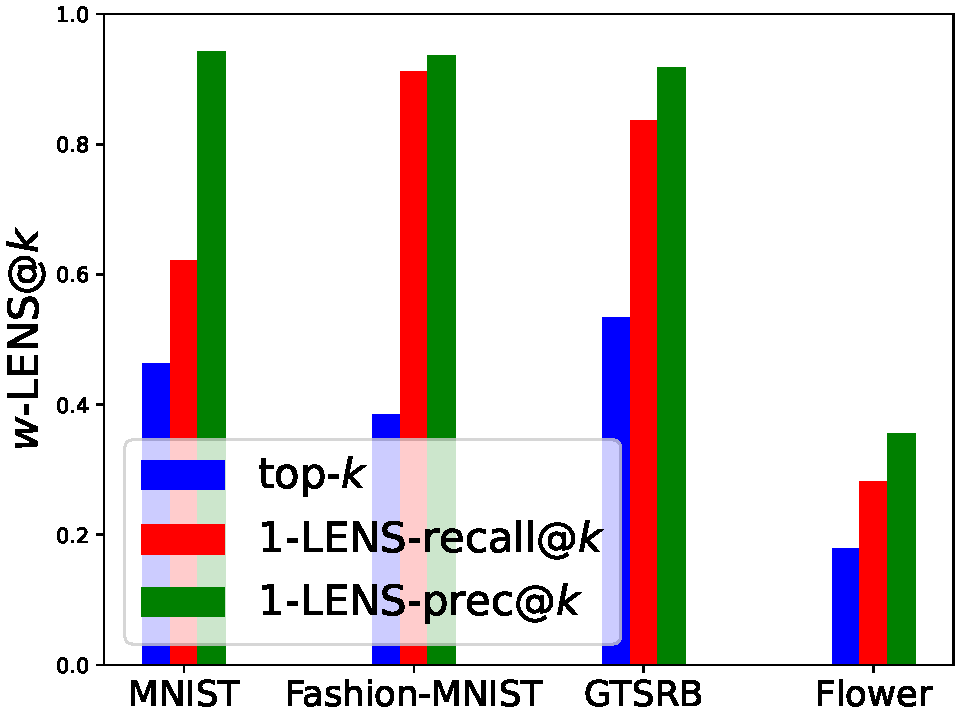
\includegraphics[width=0.25\textwidth]{./plots/datasets_topk_attack_nat_new_metric_1.pdf}
\caption{Attributional robustness of IG on naturally trained models measured as average top-$k$ intersection, $1$-LENS-prec@$k$ and $1$-LENS-recall@$k$ between IG(original image) and IG(perturbed image) obtained by the top-$t$ attack \citep{ghorbani2018interpretation} across different datasets.}
\label{dataset-topk-new-metric-st-nat}
\end{figure}

\begin{figure}[!ht]
\centering
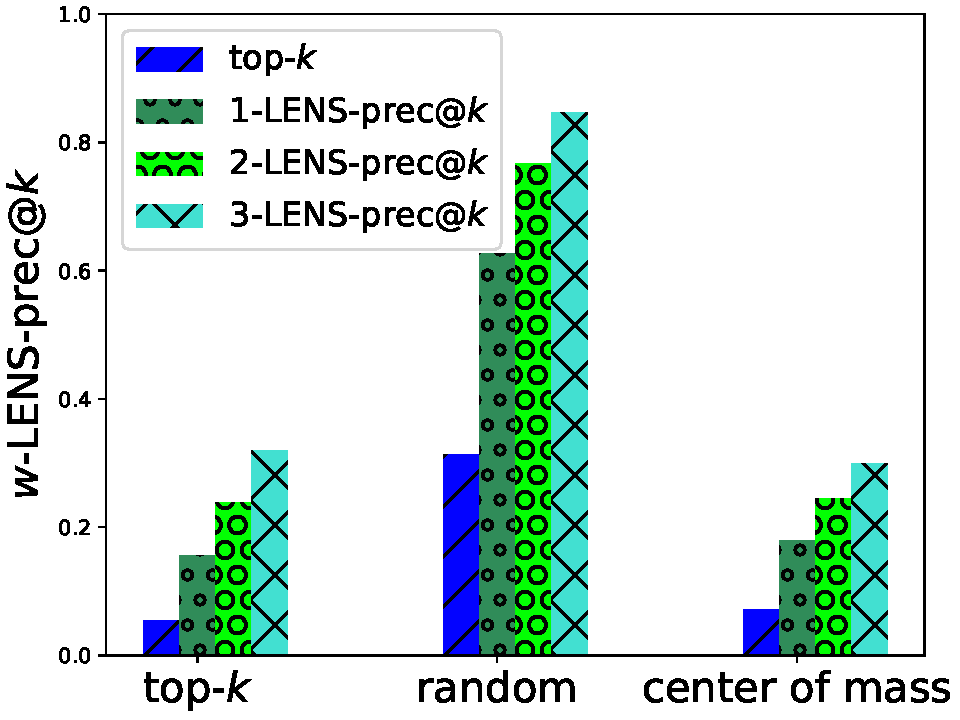
\includegraphics[width=0.22\textwidth]{./plots/imagenet_topk_attack_new_metric_nat_ig_lens.pdf}
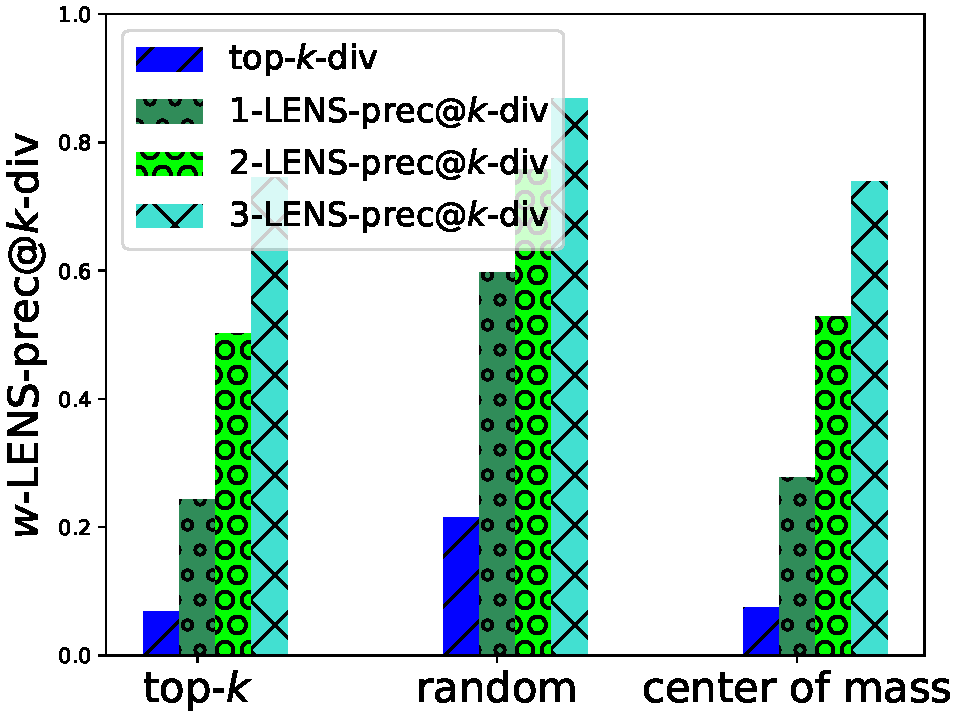
\includegraphics[width=0.219\textwidth]{./plots/imagenet_topk_attack_new_metric_nat_ig_lens_div.pdf}
\caption{Effect of increasing $w$ on average $w$-LENS-prec@$k$ and $w$-LENS-prec@$k$-div in comparison with top-$k$ intersection for IG map on ImageNet using a SqueezeNet model, when attacked with three attributional attacks (viz., top-$k$, random sign perturbation and mass center) of \citet{ghorbani2018interpretation}.}
\label{imagenet-topk-window-new-metric-nat-ig-lens}
\end{figure}

\paragraph{$w$-LENS-prec@$k$ for varying $w$.} In Figure \ref{imagenet-topk-window-new-metric-nat-ig-lens}(left) $w$-LENS-prec@$k$ increases as we increase $w$ to consider larger neighborhoods around the pixels with top attribution values. This holds for multiple perturbations, namely, top-$t$ attack and mass-center attack by \citet{ghorbani2018interpretation} as well as a random perturbation. Notice that the top-$t$ attack of \citet{ghorbani2018interpretation} is constructed specifically for the top-$t$ intersection objective, and perhaps as a result, shows larger change when we increase local-sensitivity by increasing $w$ in the robustness measure. %\textcolor{orange}{Obtained similar Figure \ref{flower-topk-window-new-metric-nat-ig} with ImageNet with LENS (Figure \ref{imagenet-topk-window-new-metric-nat-ig-lens}) and Diversity (Figure \ref{imagenet-topk-window-new-metric-nat-ig-lens-div}).}


Due to space constraint and purposes of coherence, we present few results with IG here; we present similar results on other explanation methods in the Appendix \ref{app:more-lens-results}. Refer to Appendix \ref{app:all-ig-exp} for similar plots with random sign perturbation and mass center attack of \citet{ghorbani2018interpretation}. Appendix \ref{app:all-sg-exp} contains additional results with similar conclusions when Simple Gradients are used instead of Integrated Gradients (IG) for obtaining the attributions.

As a natural follow-up question we present in Appendix \ref{app:vary-k-sp-ken} results obtained by modifying the similarity objective of top-$k$ attack of \citet{ghorbani2018interpretation} with $1$-LENS-prec@$k$ with the assumption to obtain a stronger attack. But surprisingly, we notice that it leads to a \emph{worse} attributional attack, if we measure its effectiveness using the top-$k$ intersections and $1$-LENS-prec@$k$. In other words, attributional attacks against locality-sensitive measures of attributional robustness are non-trivial and may require fundamentally different ideas.

\subsection{Alignment of attributional robustness metrics to human perception}
\label{subsec:survey-human}

We conducted a survey with human participants, where we presented images from the Flower dataset and a pair of attribution maps---an attribution map of the original image alongside an attribution map of their random perturbation or attributional attacked version \citet{ghorbani2018interpretation}, in a random order and without revealing this information to the participants. The survey participants were asked whether the two maps were relatable to the image and if one of them was different than the other. In Table \ref{table-survey-results} we summarize the results obtained from the survey. We simplify the choices presented to the user into 2 final categories - \begin{inparaenum}[(1)] \item Agree with w-LENS-prec@$k$ \item Agree with top-$k$ metric \end{inparaenum} Category (1) includes all results where the user found the maps the same, relatable to the image but dissimilar or the perturbed map was preferred over the original map. Category (2) was the case where the user preferred the original map over the perturbed map. Refer to Appendix \ref{app:survey-human} for more details.

\begin{table}[!ht]
\begin{center}
\resizebox{0.47\textwidth}{!}{
\begin{tabular}{|c|c|}
\hline
{\bf Agree with 3-LENS-prec@$k$ metric(\%)} & {\bf Agree with top-$k$ metric(\%)} \\
\hline
70.37 & 29.63 \\
\hline
\end{tabular}
}
\end{center}
\caption{Survey results based on humans ability to relate the explanation map to the original image with or without noise using the Flower dataset.}
\label{table-survey-results}
\end{table}

\begin{figure}[!ht]
  \begin{center}
    
\includegraphics[width=0.11\textwidth]{./images/flower_19_image.pdf}
    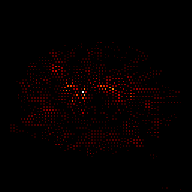
\includegraphics[width=0.11\textwidth]{./images/flower_19_topk_nat_orig_orig_div.pdf}
    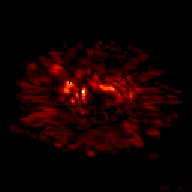
\includegraphics[width=0.11\textwidth]{./images/flower_19_topk_nat_orig_lens_rec_div.pdf}
    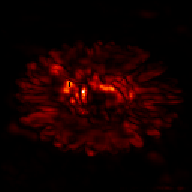
\includegraphics[width=0.11\textwidth]{./images/flower_19_topk_nat_orig_2lens_rec_div.pdf}\\
    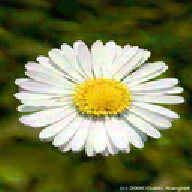
\includegraphics[width=0.11\textwidth]{./images/flower_19_image_pert.pdf}
    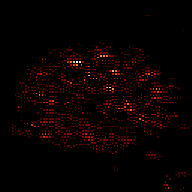
\includegraphics[width=0.11\textwidth]{./images/flower_19_topk_nat_orig_pert_div.pdf}
    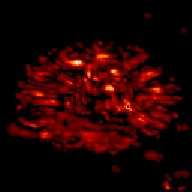
\includegraphics[width=0.11\textwidth]{./images/flower_19_topk_nat_orig_lens_pre_div.pdf}
    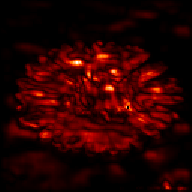
\includegraphics[width=0.11\textwidth]{./images/flower_19_topk_nat_orig_2lens_pre_div.pdf}\\
  \end{center}
      \caption{A sample image from Flower dataset before (top) and after (bottom) the top-$k$ attributional attack of \citet{ghorbani2018interpretation} on a ResNet model. For both, we show from left to right: the image, its top-$k$ diverse pixels as per IG, the union of $3 \times 3$-pixel neighborhoods and $5 \times 5$-pixel neighborhoods of the top-$k$ diverse pixels, respectively, for $k=1000$. Quantitatively, improved overlap is captured by top-$k$-div intersection: 0.22, $1$-LENS-recall@$k$-div: 0.87, $1$-LENS-pre@$k$-div: 0.86, $2$-LENS-recall@$k$-div: 0.95, $2$-LENS-pre@$k$-div: 0.93. \emph{Zoom in required to see the diverse pixels.}}
  \label{fig_intro_div-19}
\end{figure}


\section{Diverse Attribution for Robustness} \label{sec:div-lens}
Column 1 of Figure \ref{fig_intro_div-19} shows a typical  image from Flower dataset whose top-1000 pixels according to IG are concentrated in a small region. As seen in this illustrative example, when an image has multiple important parts, concentration of top attribution pixels in a small region increases vulnerability to attributional attacks. To alleviate this vulnerability, we propose post-processing any given attribution method to output top-$k$ \emph{diverse} pixels instead of just the top-$k$ pixels with the highest attribution scores. We use a natural notion of $w$-diversity based on pixel neighborhoods, so that these diverse pixels can be picked by a simple greedy algorithm. Starting with $S \leftarrow \emptyset$, repeat for $k$ steps: Pick the pixel of highest attribution score or importance outside $S$, add it to $S$ and disallow the $(2w+1) \times (2w+1)$-pixel neighborhood around it for future selection. The set of $k$ diverse pixels picked as above contains no two pixels within $(2w+1) \times (2w+1)$-pixel neighborhood of each other, and moreover, has the highest total importance (as the sum of pixel-wise attribution scores) among all such sets of $k$ pixels. The sets of $k$ pixels where no two pixels lie in $(2w+1) \times (2w+1)$-pixel neighborhood of each other form a matroid, where the optimality of greedy algorithm is well-known; see \citet{KorteLovasz1981}.

Once we have the top-$k$ diverse pixels as described above, we can extend our locality-sensitive robustness metrics from the previous section to $w$-LENS-prec@$k$-div and $w$-LENS-recall@$k$-div, defined analogously using the union of $(2w+1) \times (2w+1)$-pixel neighborhoods of top-$k$ diverse pixels. In other words, define $\tilde{S}_{k}(x)$ as the top-$k$ diverse pixels for image $x$ and $\tilde{T}_{k} = \tilde{S}_{k}(x  + \text{Att}(x))$, and use $\tilde{S_{k}}$ and $\tilde{T}_{k}$ to replace $S_{k}$ and $T_{k}$ used in Subsection \ref{subsec:define-lens}.

For $k=1000$, Figure \ref{fig_intro_div-19} shows a sample image from Flower dataset before and after the top-$k$ attributional attack of \citet{ghorbani2018interpretation}. Figure \ref{fig_intro_div-19} visually shows the top-$k$ diverse pixels in the Integrated Gradients (IG) and the union of their $(2w+1) \times (2w+1)$-pixel neighborhoods, for $w=\{1, 2\}$, for this image before and after the attributional attack. The reader may be required to zoom in to see the top-$k$ diverse pixels. See Appendix \ref{app:sample-fragility-examples} for more examples. Note that $0$-LENS-prec@$k$ and $0$-LENS-recall@$k$ are both the same and equivalent to top-$k$ intersection. However, a combined effect of locality and diversity can show a drastic leap from top-$k$ intersection value 0.14 to $2$-LENS-recall@$k$-div value 0.95 (see Fig.\ref{fig_intro_lens-19} and Fig.\ref{fig_intro_div-19}). Fig. \ref{imagenet-topk-window-new-metric-nat-ig-lens}(right) shows the effect of increasing $w$ on the $w$-LENS-prec@$k$-div metric on ImageNet.



\section{A Stronger Model for Attributional Robustness} \label{sec:adv-robust}



\begin{figure}[!ht]
  \begin{center}
    
\includegraphics[width=0.15\textwidth]{./images/flower_19_image.pdf}
    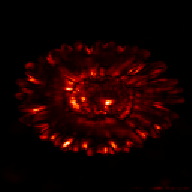
\includegraphics[width=0.15\textwidth]{./images/flower_19_topk_pgd_orig.pdf}
    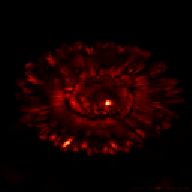
\includegraphics[width=0.15\textwidth]{./images/flower_19_topk_pgd_pert.pdf}\\
    
\includegraphics[width=0.15\textwidth]{./images/flower_19_image.pdf}
    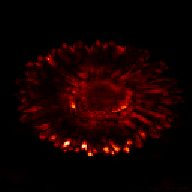
\includegraphics[width=0.15\textwidth]{./images/flower_19_topk_rar_orig.pdf}
    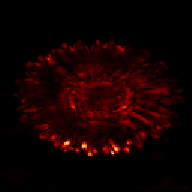
\includegraphics[width=0.15\textwidth]{./images/flower_19_topk_rar_pert.pdf}
  \end{center}
      \caption{From left to right: a sample image from Flower dataset and Integrated Gradients (IG) before and after the top-$k$ attributional attack of \citet{ghorbani2018interpretation}. The top row uses PGD-trained model whereas the bottom row uses IG-SUM-NORM-trained model.}
\label{flower-sample-pgd-rar-topk-19}
\end{figure}


A common approach to get robust attributions is to keep the attribution method unchanged but train the models differently in a way that the resulting attributions are more robust to small perturbations of inputs. \citet{chen2019robust} proposed the first defense against the attributional attack of \citet{ghorbani2018interpretation}. \citet{wang2020smoothed} also find that IG-NORM based training of \citet{chen2019robust} gives models that exhibit attributional robustness against the top-$k$ attack of \citet{ghorbani2018interpretation} along with adversarially trained models. Figure \ref{flower-sample-pgd-rar-topk-19} shows a sample image from the Flower dataset, where the Integrated Gradients (IG) of the original image and its perturbation by the top-$k$ attack are visually similar for models that are either adversarially trained (trained using Projected Gradient Descent or PGD-trained, as proposed by \citep{madry2019deep}) or IG-SUM-NORM trained as in \citet{chen2019robust}. In other words, these differently trained model guard the sample image against the attributional top-$k$ attack. Recent work by \citet{nourelahi2022} has empirically studied the effectiveness of adversarially (PGD) trained models in obtaining better attributions, e.g., Figure \ref{flower-sample-pgd-rar-topk-19}(center) shows sharper attributions to features highlighting the ground-truth class.

\begin{figure}[!ht]
\centering
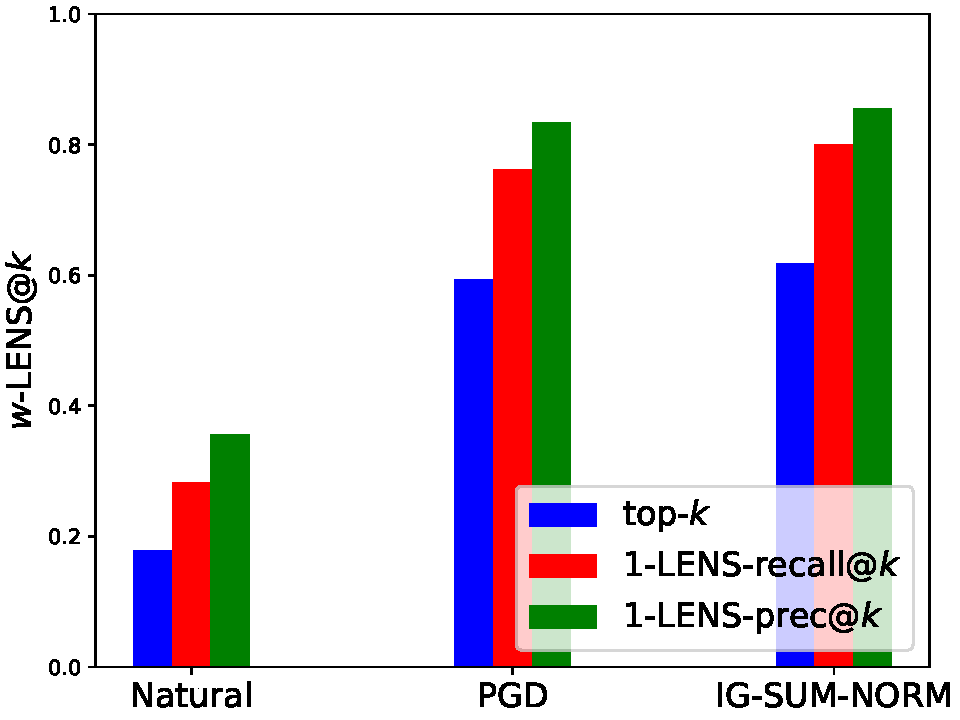
\includegraphics[width=0.219\textwidth]{./plots/flower_topk_3x3_attack_new_metric_1.pdf}
\caption{For Flower dataset, average top-$k$ intersection, $1$-LENS-prec@$k$, $1$-LENS-recall@$k$ measured between IG(original image) and IG(perturbed image) for models that are naturally trained, PGD-trained and IG-SUM-NORM trained. The perturbation used is the top-$t$ attack of \cite{ghorbani2018interpretation}. Note top-$k$ is equivalent to $0$-LENS-prec@$k$, $0$-LENS-recall@$k$.}
\label{flower-nat-pgd-rar-ig-diff-lens}
\end{figure}



Figure \ref{flower-nat-pgd-rar-ig-diff-lens} shows that PGD-trained and IG-SUM-NORM trained models have more robust Integrated Gradients (IG) in comparison to their naturally trained counterparts, and this holds for the previously used measures of attributional robustness (e.g., top-$k$ intersection) as well as the new locality-sensitive measures we propose (e.g., $1$-LENS-prec@$k$, $1$-LENS-recall@$k$) across all datasets in \citet{chen2019robust} experiments (Refer Appendix \ref{app:all-ig-exp} and \ref{app:all-sg-exp}). The top-$k$ attack of \citet{ghorbani2018interpretation} is not a threat to IG if we simply measure its effectiveness using $1$-LENS-prec@$k$ (Appendix \ref{app:all-ig-exp}, \ref{app:all-sg-exp} for MNIST, Fashion MNIST and GTSRB). The above observation about robustness of Integrated Gradients (IG) for PGD-trained and IG-SUM-NORM trained models holds even when we use $1$-LENS-Spearman and $1$-LENS-Kendall measures to quantify the attributional robustness to the top-$k$ attack of \citet{ghorbani2018interpretation}, and it holds across the datasets used by \citet{chen2019robust} in their study; see Appendix \ref{app:more-lens-results}.


\citet{ChalasaniC00J20} show theoretically that $\ell_{\infty}$-adversarial training (PGD-training) leads to stable Integrated Gradients (IG) under $\ell_{1}$ norm. They also show empirically that PGD-training leads to sparse attributions (IG \& DeepSHAP) when sparseness in measured indirectly as the change in Gini index. Our empirical results extend their theoretical observation about stability of IG for PGD-trained models, as we measure local stability in terms of both the top attribution values and their positions in the image.

Table \ref{table-topk-div-results-rand-imagenet} obtains the top-$k$ intersection, 3-LENS-recall@$k$, and 3-LENS-recall@$k$-div of different attribution methods on ImageNet for naturally trained and PGD-trained ResNet50 models. We observe that for random sign attack the improvement obtained on top-$k$ intersection is reduced for a large dataset like ImageNet. Still our conclusions about locality and diversity in attribution robustness in comparison with the top-$k$ intersection baseline holds as we observe improvements in using diversity and locality.
More results about incorporating diversity in the attribution and the resulting robustness metrics are available in Appendix \ref{app:extra-div-results}.

\begin{table}[!ht]
\begin{center}
\resizebox{0.47\textwidth}{!}{
\begin{tabular}{|l|l|c|c|c|}
\hline
{\bf Training} & {\bf Attribution method} & {\bf top-$k$} & {\bf 3-LENS-recall@$k$} & {\bf 3-LENS-recall@$k$-div} \\
\hline
Natural & Simple Gradient       & 0.3825 & 0.7875 & 0.8290 \\
Natural & Image $\times$ Gradient  & 0.3316 & 0.7765 & 0.8655 \\
Natural & LRP [Bach 2015]     & 0.1027 & 0.2487 & 0.7518 \\
Natural & DeepLIFT [Shrikumar 2017] & 0.2907 & 0.7641 & 0.8504 \\
Natural & GradSHAP [Lundberg 2017] & 0.2290 & 0.6513 & 0.8099 \\
Natural & IG [Sundararajan 2017]      & 0.2638 & 0.7148 & 0.8380 \\
\hline
PGD & Simple Gradient       & 0.1725 & 0.7245 & 0.8004 \\
PGD & Image $\times$ Gradient      & 0.1714 & 0.7269 & 0.8552 \\
PGD & LRP [Bach 2015] & 0.2374 & 0.4147 & 0.8161 \\
PGD & DeepLIFT [Shrikumar 2017] & 0.5572 & 0.9746 & 0.8977 \\
PGD & GradSHAP [Lundberg 2017] & 0.1714 & 0.7270 & 0.8552 \\
PGD & IG [Sundararajan 2017]      & 0.1947 & 0.7335 & 0.8584 \\
\hline
\end{tabular}
}
\caption{Average top-$k$ intersection, 3-LENS-prec@$k$ and 3-LENS-prec@$k$-div for random sign perturbation attack applied to different attribution methods on ImageNet for naturally and adversarially(PGD)-trained ResNet50 models.}
\label{table-topk-div-results-rand-imagenet}
\end{center}
\end{table}

\section{Conclusion and Future Work} \label{sec:conclusion}
We show that the fragility of attributions is an effect of using fragile robustness metrics such as top-$k$ intersection that only look at the rank order of attributions and fail to capture the locality of pixel positions with high attributions. We highlight the need for locality-sensitive metrics for attributional robustness and propose natural locality-sensitive extensions of existing metrics. We introduce another method of picking diverse top-$k$ pixels that can be naturally extended with locality to obtain improved measure of attributional robustness. Theoretical understanding of locality-sensitive metrics of attributional robustness, constructing stronger attributional attacks for these metrics, and using them to build attributionally robust models are important future directions.


Magni omnis nam perferendis at exercitationem nesciunt asperiores numquam, dolorum fugiat repudiandae veniam laborum eveniet reiciendis, corporis quos rem neque consequatur dolores in velit quae, id ex reiciendis ipsum, eligendi accusamus a?Maxime eligendi repellat molestiae numquam atque quaerat laudantium, assumenda ipsam ipsa nemo non, eius odit officia quas voluptates, magni unde officia vero excepturi dolor minima quas aliquam quam molestias asperiores?Ex voluptas reiciendis, assumenda culpa maiores veritatis perspiciatis voluptas dolores nesciunt praesentium quia qui aliquid, eveniet molestiae mollitia enim, quod accusamus nulla?Deleniti omnis in doloribus repudiandae, tempora laborum obcaecati ratione repellendus, laudantium perspiciatis modi velit, sit nihil exercitationem praesentium quibusdam tenetur, delectus minus temporibus.Dolore ipsum asperiores rem vitae culpa beatae earum, eius laboriosam vitae, voluptates amet dolore officiis pariatur beatae nisi a, eos distinctio atque aperiam voluptatum eveniet necessitatibus asperiores minima aut porro?Suscipit perspiciatis assumenda ipsam repudiandae ab unde iusto tempora, voluptates minus delectus ipsa earum quia mollitia unde alias harum hic quisquam.Molestiae ipsam tempore dignissimos cumque earum laborum possimus corporis itaque ad, excepturi veniam aspernatur?Non similique vitae ipsa, veniam sed totam molestiae ab porro deserunt quibusdam cum perspiciatis laboriosam, nam a modi ad quia placeat alias rem similique debitis expedita, odio numquam eaque corrupti doloribus nobis fugiat sed laborum quaerat, numquam expedita voluptatem non fugit sunt officia laudantium perferendis?Ullam vero at mollitia cumque provident illum esse totam quo perspiciatis aliquam, voluptatem ducimus doloribus aperiam eveniet, aliquam libero nostrum totam ex voluptatum labore quos nihil reiciendis ut adipisci, in omnis laboriosam expedita quis minus est error ullam nulla laborum?Soluta excepturi architecto quas ex laboriosam suscipit corrupti nihil tempore nobis laborum, harum repellendus temporibus ipsum ipsa quas iusto, hic culpa illum, minima iusto cupiditate illum tempore maiores sint commodi aliquid necessitatibus, accusamus repudiandae quisquam ratione hic?Fugit consequuntur adipisci sunt est, ipsa sed nesciunt delectus adipisci modi magni qui quam inventore ipsam, hic rerum temporibus nesciunt eveniet, nihil minus nisi voluptatem modi, necessitatibus magni ut quam pariatur debitis eveniet laborum?Labore laudantium vitae ipsum, totam velit quisquam, reprehenderit tempora voluptatum repudiandae cum reiciendis quam deleniti tenetur ducimus accusantium maiores, tempore ullam assumenda doloremque ipsam nemo provident tempora perferendis quos, molestias fuga
\bibliography{anonymous-submission-latex-2024}
\bibliographystyle{aaai24}



\end{document}